\section{user Class Reference}
\label{classuser}\index{user@{user}}
user plugin  


Inheritance diagram for user::\begin{figure}[H]
\begin{center}
\leavevmode
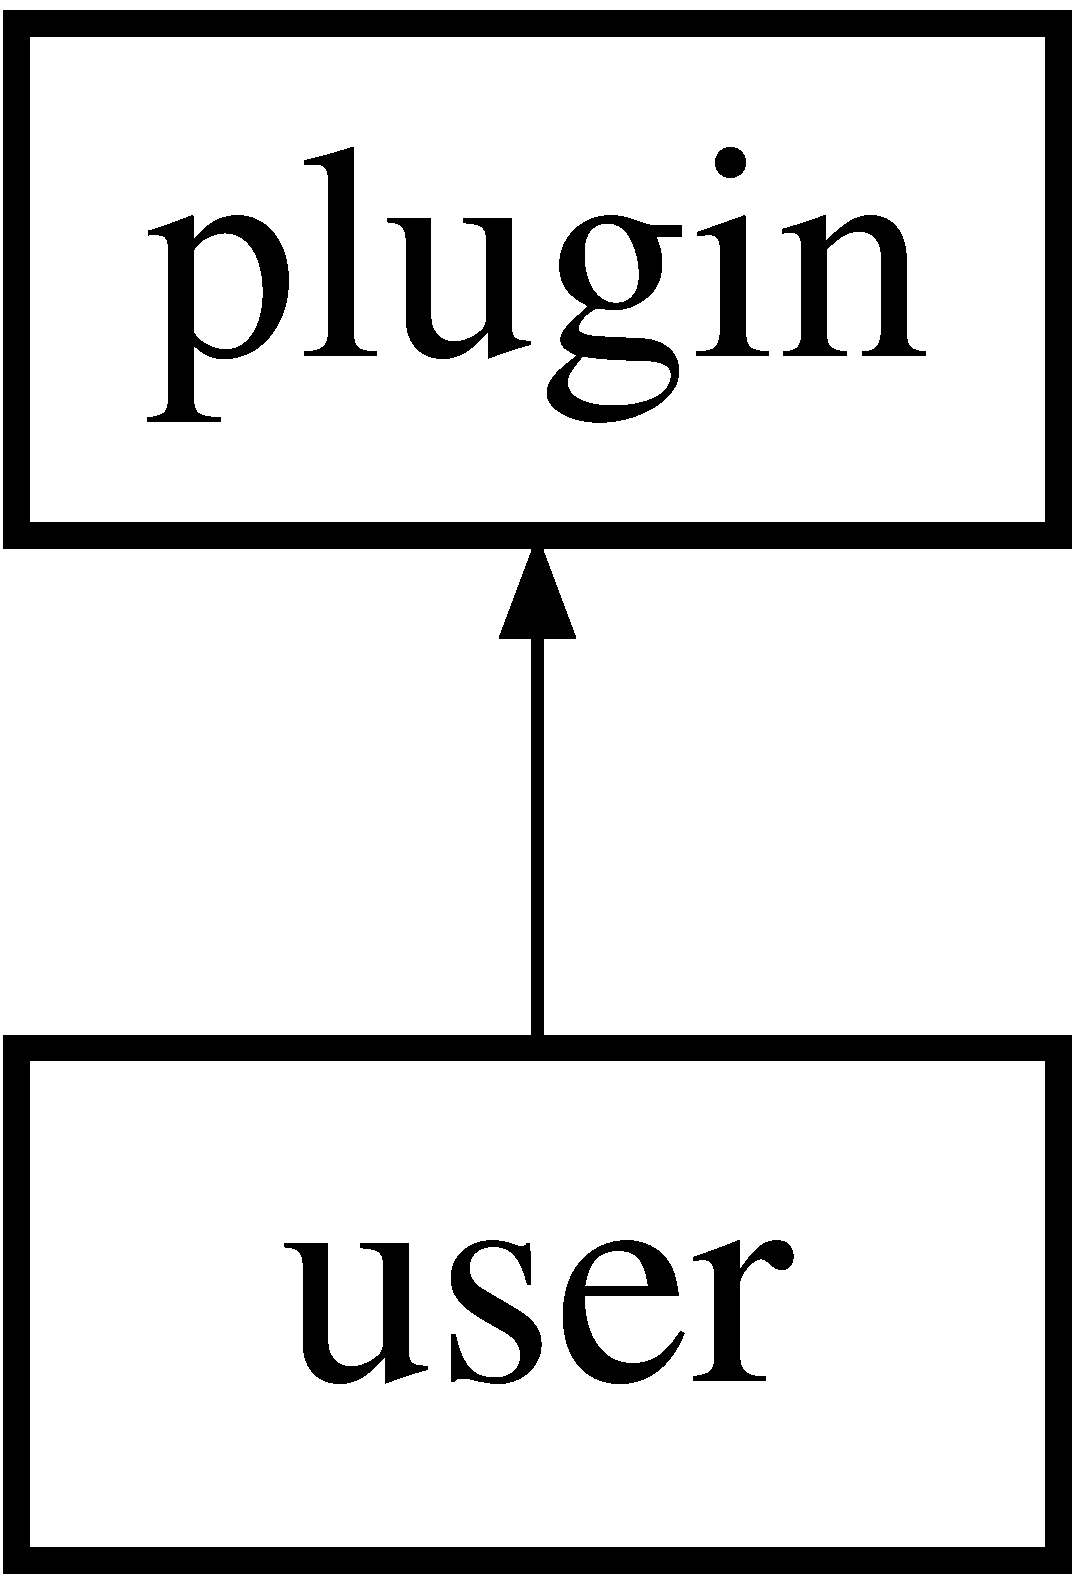
\includegraphics[height=2cm]{classuser}
\end{center}
\end{figure}
\subsection*{Public Member Functions}
\begin{CompactItemize}
\item 
{\bf user} (\${\bf dn}=NULL)\label{classuser_a0}

\item 
{\bf execute} ()
\begin{CompactList}\small\item\em execute plugin \item\end{CompactList}\item 
{\bf remove\_\-from\_\-parent} ()\label{classuser_a2}

\item 
{\bf save\_\-object} ()\label{classuser_a3}

\item 
{\bf save} ()\label{classuser_a4}

\item 
{\bf check} ()\label{classuser_a5}

\end{CompactItemize}
\subsection*{Public Attributes}
\begin{CompactItemize}
\item 
{\bf base} = \char`\"{}\char`\"{}\label{classuser_o0}

\item 
{\bf cn} = \char`\"{}\char`\"{}\label{classuser_o1}

\item 
{\bf personal\-Title} = \char`\"{}\char`\"{}\label{classuser_o2}

\item 
{\bf academic\-Title} = \char`\"{}\char`\"{}\label{classuser_o3}

\item 
{\bf home\-Postal\-Address} = \char`\"{}\char`\"{}\label{classuser_o4}

\item 
{\bf home\-Phone} = \char`\"{}\char`\"{}\label{classuser_o5}

\item 
{\bf labeled\-URI} = \char`\"{}\char`\"{}\label{classuser_o6}

\item 
{\bf o} = \char`\"{}\char`\"{}\label{classuser_o7}

\item 
{\bf ou} = \char`\"{}\char`\"{}\label{classuser_o8}

\item 
{\bf department\-Number} = \char`\"{}\char`\"{}\label{classuser_o9}

\item 
{\bf employee\-Number} = \char`\"{}\char`\"{}\label{classuser_o10}

\item 
{\bf employee\-Type} = \char`\"{}\char`\"{}\label{classuser_o11}

\item 
{\bf room\-Number} = \char`\"{}\char`\"{}\label{classuser_o12}

\item 
{\bf telephone\-Number} = \char`\"{}\char`\"{}\label{classuser_o13}

\item 
{\bf facsimile\-Telephone\-Number} = \char`\"{}\char`\"{}\label{classuser_o14}

\item 
{\bf mobile} = \char`\"{}\char`\"{}\label{classuser_o15}

\item 
{\bf pager} = \char`\"{}\char`\"{}\label{classuser_o16}

\item 
{\bf l} = \char`\"{}\char`\"{}\label{classuser_o17}

\item 
{\bf st} = \char`\"{}\char`\"{}\label{classuser_o18}

\item 
{\bf postal\-Address} = \char`\"{}\char`\"{}\label{classuser_o19}

\item 
{\bf jpeg\-Photo} = \char`\"{}$\ast$removed$\ast$\char`\"{}\label{classuser_o20}

\item 
{\bf photo\-Data} = \char`\"{}\char`\"{}\label{classuser_o21}

\item 
{\bf old\_\-jpeg\-Photo} = \char`\"{}\char`\"{}\label{classuser_o22}

\item 
{\bf old\_\-photo\-Data} = \char`\"{}\char`\"{}\label{classuser_o23}

\item 
{\bf cert\_\-dialog} = FALSE\label{classuser_o24}

\item 
{\bf picture\_\-dialog} = FALSE\label{classuser_o25}

\item 
{\bf user\-PKCS12} = \char`\"{}\char`\"{}\label{classuser_o26}

\item 
{\bf user\-SMIMECertificate} = \char`\"{}\char`\"{}\label{classuser_o27}

\item 
{\bf user\-Certificate} = \char`\"{}\char`\"{}\label{classuser_o28}

\item 
{\bf certificate\-Serial\-Number} = \char`\"{}\char`\"{}\label{classuser_o29}

\item 
{\bf old\_\-certificate\-Serial\-Number} = \char`\"{}\char`\"{}\label{classuser_o30}

\item 
{\bf old\_\-user\-PKCS12} = \char`\"{}\char`\"{}\label{classuser_o31}

\item 
{\bf old\_\-user\-SMIMECertificate} = \char`\"{}\char`\"{}\label{classuser_o32}

\item 
{\bf old\_\-user\-Certificate} = \char`\"{}\char`\"{}\label{classuser_o33}

\item 
{\bf gouvernment\-Organizational\-Unit} = \char`\"{}\char`\"{}\label{classuser_o34}

\item 
{\bf house\-Identifier} = \char`\"{}\char`\"{}\label{classuser_o35}

\item 
{\bf street} = \char`\"{}\char`\"{}\label{classuser_o36}

\item 
{\bf postal\-Code} = \char`\"{}\char`\"{}\label{classuser_o37}

\item 
{\bf vocation} = \char`\"{}\char`\"{}\label{classuser_o38}

\item 
{\bf ivbb\-Last\-Delivery\-Collective} = \char`\"{}\char`\"{}\label{classuser_o39}

\item 
{\bf gouvernment\-Organizational\-Person\-Locality} = \char`\"{}\char`\"{}\label{classuser_o40}

\item 
{\bf gouvernment\-Organizational\-Unit\-Description} = \char`\"{}\char`\"{}\label{classuser_o41}

\item 
{\bf gouvernment\-Organizational\-Unit\-Subject\-Area} = \char`\"{}\char`\"{}\label{classuser_o42}

\item 
{\bf functional\-Title} = \char`\"{}\char`\"{}\label{classuser_o43}

\item 
{\bf role} = \char`\"{}\char`\"{}\label{classuser_o44}

\item 
{\bf public\-Visible} = \char`\"{}\char`\"{}\label{classuser_o45}

\item 
{\bf pw\_\-storage} = \char`\"{}crypt\char`\"{}\label{classuser_o46}

\item 
{\bf last\_\-pw\_\-storage} = \char`\"{}crypt\char`\"{}\label{classuser_o47}

\item 
{\bf attributes}
\item 
{\bf objectclasses} = array(\char`\"{}person\char`\"{}, \char`\"{}organizational\-Person\char`\"{}, \char`\"{}inet\-Org\-Person\char`\"{}, \char`\"{}gosa\-Account\char`\"{})\label{classuser_o49}

\end{CompactItemize}


\subsection{Detailed Description}
user plugin 

\begin{Desc}
\item[Author:]Cajus Pollmeier $<${\tt pollmeier@gonicus.de}$>$ \end{Desc}
\begin{Desc}
\item[Version:]2.00 \end{Desc}
\begin{Desc}
\item[Date:]24.07.2003\end{Desc}
This class provides the functionality to read and write all attributes relevant for person, organizational\-Person, inet\-Org\-Person and gosa\-Account from/to the LDAP. It does syntax checking and displays the formulars required. 



\subsection{Member Function Documentation}
\index{user@{user}!execute@{execute}}
\index{execute@{execute}!user@{user}}
\subsubsection{\setlength{\rightskip}{0pt plus 5cm}user::execute ()}\label{classuser_a1}


execute plugin 

Generates the html output for this node 

Reimplemented from {\bf plugin} {\rm (p.\,\pageref{classplugin_a1})}.

\subsection{Member Data Documentation}
\index{user@{user}!attributes@{attributes}}
\index{attributes@{attributes}!user@{user}}
\subsubsection{\setlength{\rightskip}{0pt plus 5cm}user::attributes}\label{classuser_o48}


{\bf Initial value:}

\footnotesize\begin{verbatim} array("sn", "givenName", "uid", "personalTitle", "academicTitle",
        "homePostalAddress", "homePhone", "labeledURI", "o", "ou",
        "departmentNumber", "employeeNumber", "employeeType", "l", "st",
        "roomNumber", "telephoneNumber", "mobile", "pager", "cn", "userPKCS12",
        "postalAddress", "facsimileTelephoneNumber", "userSMIMECertificate",
        "gouvernmentOrganizationalUnit", "houseIdentifier", "vocation",
        "ivbbLastDeliveryCollective", "gouvernmentOrganizationalPersonLocality",
        "gouvernmentOrganizationalUnitDescription", "postalCode", "street",
        "gouvernmentOrganizationalUnitSubjectArea", "functionalTitle",
        "role", "certificateSerialNumber", "publicVisible")
\end{verbatim}\normalsize 


Reimplemented from {\bf plugin} {\rm (p.\,\pageref{classplugin})}.

The documentation for this class was generated from the following file:\begin{CompactItemize}
\item 
class\_\-user.inc\end{CompactItemize}
